% This file was created with tikzplotlib v0.10.1.
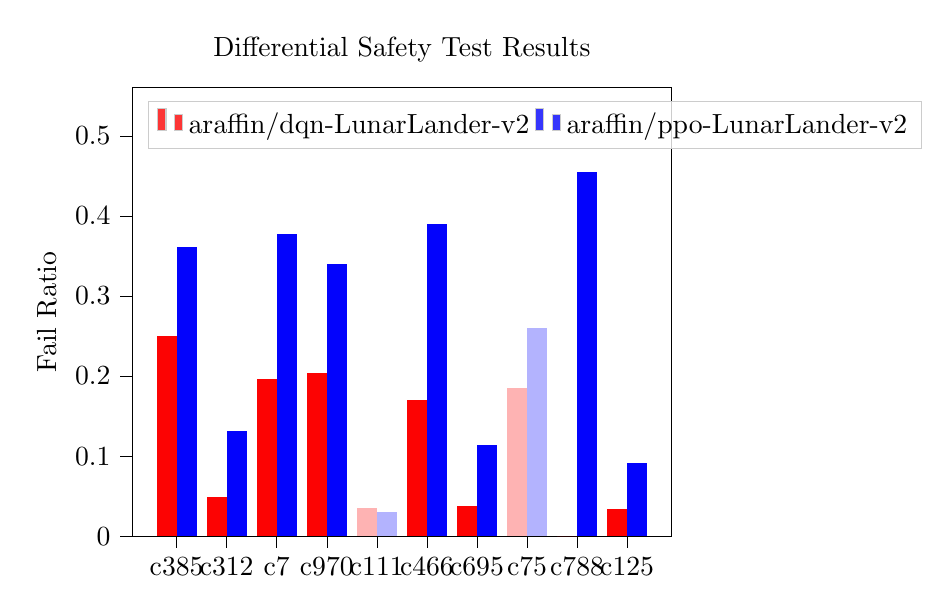
\begin{tikzpicture}

\definecolor{blue33252}{RGB}{3,3,252}
\definecolor{darkgray176}{RGB}{176,176,176}
\definecolor{lightgray204}{RGB}{204,204,204}
\definecolor{red25233}{RGB}{252,3,3}

\begin{axis}[
legend cell align={left},
legend columns=3,
legend style={
  fill opacity=0.8,
  draw opacity=1,
  text opacity=1,
  at={(0.03,0.97)},
  anchor=north west,
  draw=lightgray204
},
tick align=outside,
tick pos=left,
title={Differential Safety Test Results},
x grid style={darkgray176},
xmin=-0.49, xmax=10.29,
xtick style={color=black},
xtick={0.4,1.4,2.4,3.4,4.4,5.4,6.4,7.4,8.4,9.4},
xticklabels={c385,c312,c7,c970,c111,c466,c695,c75,c788,c125},
y grid style={darkgray176},
ylabel={Fail Ratio},
ymin=0, ymax=0.56,
ytick style={color=black}
]
\draw[draw=none,fill=red25233] (axis cs:-2.77555756156289e-17,0) rectangle (axis cs:0.4,0.25);
\addlegendimage{ybar,ybar legend,draw=none,fill=red25233}
\addlegendentry{araffin/dqn-LunarLander-v2}

\draw[draw=none,fill=red25233] (axis cs:1,0) rectangle (axis cs:1.4,0.0491803278688525);
\draw[draw=none,fill=red25233] (axis cs:2,0) rectangle (axis cs:2.4,0.19672131147541);
\draw[draw=none,fill=red25233] (axis cs:3,0) rectangle (axis cs:3.4,0.203883495145631);
\draw[draw=none,fill=red25233] (axis cs:5,0) rectangle (axis cs:5.4,0.170731707317073);
\draw[draw=none,fill=red25233] (axis cs:6,0) rectangle (axis cs:6.4,0.0378787878787879);
\draw[draw=none,fill=red25233] (axis cs:8,0) rectangle (axis cs:8.4,0);
\draw[draw=none,fill=red25233] (axis cs:9,0) rectangle (axis cs:9.4,0.0342857142857143);
\draw[draw=none,fill=blue33252] (axis cs:0.4,0) rectangle (axis cs:0.8,0.361842105263158);
\addlegendimage{ybar,ybar legend,draw=none,fill=blue33252}
\addlegendentry{araffin/ppo-LunarLander-v2}

\draw[draw=none,fill=blue33252] (axis cs:1.4,0) rectangle (axis cs:1.8,0.131147540983607);
\draw[draw=none,fill=blue33252] (axis cs:2.4,0) rectangle (axis cs:2.8,0.377049180327869);
\draw[draw=none,fill=blue33252] (axis cs:3.4,0) rectangle (axis cs:3.8,0.339805825242718);
\draw[draw=none,fill=blue33252] (axis cs:5.4,0) rectangle (axis cs:5.8,0.390243902439024);
\draw[draw=none,fill=blue33252] (axis cs:6.4,0) rectangle (axis cs:6.8,0.113636363636364);
\draw[draw=none,fill=blue33252] (axis cs:8.4,0) rectangle (axis cs:8.8,0.454545454545455);
\draw[draw=none,fill=blue33252] (axis cs:9.4,0) rectangle (axis cs:9.8,0.0914285714285714);
\draw[draw=none,fill=red25233,fill opacity=0.3] (axis cs:4,0) rectangle (axis cs:4.4,0.035);
\draw[draw=none,fill=red25233,fill opacity=0.3] (axis cs:7,0) rectangle (axis cs:7.4,0.185);
\draw[draw=none,fill=blue33252,fill opacity=0.3] (axis cs:4.4,0) rectangle (axis cs:4.8,0.03);
\draw[draw=none,fill=blue33252,fill opacity=0.3] (axis cs:7.4,0) rectangle (axis cs:7.8,0.26);
\end{axis}

\end{tikzpicture}
